\usepackage[authoryear,round]{natbib}
\usepackage{multirow}

\newcommand{\sheetnum}{%
	15
}
%\setcounter{section}{\sheetnum-3}
\newcommand{\tutorialtitle}{%
    Reinforcement Learning Pt 2/2 
    (Q-Learning)
}
\newcommand{\tutorialtitleshort}{%
	RL (Q-Learning)
}
% for slides
\subtitle{\sheetnum \tutorialtitle}

\maxdeadcycles=1000 % Workaround for ! Output loop---100 consecutive dead cycles because of too many figures

% The following use of algroithms does not work well with the notes:
%
%
%
%
% instead use the following for your algorithms:
%
%\begin{figure}[!t]
%\removelatexerror
%\begin{algorithm}[H]
    % your algo here
    %\label{alg:algolabel}
    %\caption{algocaption}
%\end{algorithm}
%\end{figure}
%\begin{algorithm}
% Below is the definition for the command \removelatexerror:
\makeatletter
\newcommand{\removelatexerror}{\let\@latex@error\@gobble}
\makeatother

\begin{document} %%%%%%%%%%%%%%%%%%%%%%%%%%%%%%%%%%%%%%%%%%%%%%%%%%%%%%%

\sheet{\sheetnum}{\tutorialtitleshort}

\ttopic{\tutorialtitle}

\columnratio{0.2,0.8}\textbf{}
\begin{paracol}{2}
%\setlength{\columnseprule}{0.1pt}
%\setlength{\columnsep}{5em}

\begin{rightcolumn}

% notes version will ignore it
\begin{frame}
\titlepage
\end{frame}

\begin{frame}
\tableofcontents
\end{frame}

\newpage

\mode<all>
\section{Recap of Markov Decision Process (MDP)}

\definecolor{reward}{rgb}{0,0.5,0}
\definecolor{policy}{rgb}{0.75,0,0}
\definecolor{trans}{rgb}{0,0,1}

\begin{frame}\frametitle{\secname}

\begin{itemize}
\item[] states $\vec x \in \mathcal{X} = \{ \vec x_1, \ldots, \vec x_S\}$
\item[] actions $\vec a \in \mathcal{A} = \{ \vec a_1, \ldots, \vec a_A\}$
\item[] transition model
$$P(\vec x_j | \vec x_i, \vec a_k)$$
\pause
\item[] reward function
$$r(\vec x_i, \vec a_k)$$
\item[] policy
$$
\pi(\vec a_k | \vec x_i)$$
\end{itemize}

\end{frame}

\begin{frame}\frametitle{Recap (cont'd)}

The value function to evaluate a policy:

	\begin{align}
	V^\pi(\vec x_i) =
	\E \bigg\lbrack
	\sum_{t=0}^{\infty} \gamma^t r(\vec x^{(t)}, \vec a^{(t)}) \;\Big|\; \vec x^{(0)} := \vec x_i
	\bigg\rbrack\,, \; i=1,\ldots,S
	\end{align}
	
	\mode<article>{
	$\E\lbrack\cdot\rbrack$ is w.r.t $\{\vec x^{(t)}, \vec a^{(t)}\}$
	}
	
Comparing policies:

\begin{equation}
\pi~
\overset{\mathclap{\substack{%
					\text{``better'' or}\\[1mm]\text{equally ``good''}\\ \big\downarrow
					}}}{{\color{gray}\ge}}
~\pi' 
\quad \text{\textbf{iff}} \quad V^{\pi} (\vec x) \ge V^{\pi'} (\vec x)\,,\quad \forall\; \vec x \in \mathcal{X}
\end{equation}

The optimal value function and optimal policies:

\begin{equation}
\underbrace{V^{*}(\vec x)}_{\substack{\text{optimal}\\ \text{value}}}
\;\;=\;\; \max_{\pi} V^{\pi} (\vec x)
\;\;=\;\; \underbrace{V^{\pi*}(\vec x)}_{\mathclap{\substack{\text{value of}\\ \text{optimal policy}}}}\,,\quad \forall \vec x \in \mathcal{X}
\end{equation}

\end{frame}



\mode*

\clearpage

\mode<all>
\section{Model-free evaluation of policy}

\newcommand{\lr}{\eta}

\begin{frame} 
\mode<presentation>{
    \begin{center} \huge
        \secname
    \end{center}  
    }
    \begin{center}
    \underline{Last time}: Model-based $\corresponds$ offline-planning.\\
    \underline{Today}: Model-free $\corresponds$ inductive online-planning.\\
    \end{center}
\end{frame}

\begin{frame}\frametitle{\secname}

Motivation for model-free evaluation methods:\\

\slidesonly{\vspace{5mm}}

The MDP is not explicitly available, i.e. \notesonly{\textcolor{trans}the transition model }${\color{trans}P}$ and \notesonly{\textcolor{reward}the reward function }${\color{reward}r}$ are unknown and have to be ``experienced''.\\

\slidesonly{\vspace{5mm}}

Options:
\begin{enumerate}[A]
\item Monte-Carlo estimation of $V^\pi(\vec x)$
\item Inductive value estimation through temporal difference learning (TD-Learning)
\end{enumerate}

\end{frame}

\subsection{Monte-Carlo estimation of the value function}

\begin{frame}\frametitle{Model-free option A:~\subsecname}

Monte-Carlo estimation:

	\begin{itemize}
		\item sampling of sequences: step-by-step construction of states, actions and rewards to form possible markov chains
		\item We deal with a finite approximation of infinite Markov chains. This implies:
			\begin{itemize}
				\item rewards weighted by $\gamma^H < \epsilon$ are neglected
				\item value is the discounted reward \textbf{averaged} over $n$ Markov chains of length $H$. \notesonly{This averaging is what leads to the estimates of the state values.}
			\end{itemize}
		
		\question{What are your thoughts about the efficiency of Monte-Carlo estimation?}
		
		\pause 
		
		\item Monte-Carlo estimation requires drawing $n$ chains 
			from the same initial state %$\vec x^{(0)}$
		\item $n$ must be sufficiently large
		\item every state must be evaluated often 
			$\leadsto$ not sample efficient
	\end{itemize}
	
\end{frame}

\subsubsection{Inductive value estimation}

\begin{frame}\frametitle{\subsecname:~\subsubsecname}

	Recall the Bellman equation:
	\begin{equation}
			V^\pi(\vec x_i) \;\;=\;\;
				{\color{policy} \smallsum{k=1}A 
					\pi(\vec a_k \,|\, \vec x_i)}~ 
					{\color{reward} r(\vec x_i, \vec a_k)}
				\;+\; \gamma {\color{trans} \smallsum{j=1}{S}}
					{\color{policy} \smallsum{k=1}A 
					\pi(\vec a_k \,|\, \vec x_i)}~
					{\color{trans} P(\vec x_j \,|\, \vec x_i, \vec a_k)} V^\pi(\vec x_j)
	\end{equation}
		
	\begin{itemize}
		\item But the reward, ${\color{reward} r(\vec x_i, \vec a_k)}$, and the transition model, ${\color{trans}P(\vec  x_j | \vec  x_i, \vec  a_k)}$
		 may not be available to the agent (motivation for model-free evaluation)
		 
		 \pause
		 
		 \slidesonly{\vspace{5mm}}
		 
		\item Inductive value estimation: \underline{Estimating} the value function by sampling from one long Markov chain, i.e.
			\begin{enumerate}
				\item actions are drawn according to the {\color{policy}policy} 
				$ \vec a^{(t)} \sim {\color{policy}\pi(\cdot|\, \vec x^{(t)})}$
				
				\item which lead to {\color{trans}transitions} 
					${\color{trans}\vec x^{(t+1)}
					\sim P(\cdot|\vec x^{(t)},\vec a^{(t)})}$
					
				\item and yield immediate {\color{reward} rewards 
					$r(\vec x^{(t)},\vec a^{(t)})$}
			\end{enumerate}
	\end{itemize}
	
\end{frame}

\mode<presentation>{
\begin{frame}\frametitle{\secname}

Options:
\begin{enumerate}[A]
\item \textcolor{gray}{Monte-Carlo estimation of $V^\pi(\vec x)$}
\item Inductive value estimation through temporal difference learning (TD learning)
\end{enumerate}

\end{frame}
}

\subsection{Temporal difference (TD) learning}

% -----------------------------------------------------------------------------
\begin{frame}\frametitle{Model-free option B:~\subsecname}

%\notesonly{
Temporal difference learning (TD learning) is also a form of inductive value estimation.
%}

\mode<presentation>{
		\begin{enumerate}
			\item actions are drawn according to the {\color{policy}policy} 
		 	$ \vec a^{(t)} \sim {\color{policy}\pi(\cdot|\, \vec x^{(t)})}$
		 	
			\item which lead to {\color{trans}transitions} 
		 		${\color{trans}\vec x^{(t+1)}
		 		\sim P(\cdot|\vec x^{(t)},\vec a^{(t)})}$
		 		
			\item and yield immediate {\color{reward} rewards 
		 		$r(\vec x^{(t)},\vec a^{(t)}) =: r{(t)}$}
		\end{enumerate}
}

\pause 

\vspace{2mm}

TD learning is the asynchronous on-line update of the value function one state at a time
	\slidesonly{\vspace{-8mm}}
	
	\begin{equation}
		\tilde V^{\pi}_{(t+1)}(\vec x^{(t)}) \; = \; 
		\tilde V^{\pi}_{(t)}(\vec x^{(t)}) \;+\;
		\lr \Big( \underbrace{{\color{reward}r^{(t)}} 
		+ \overbrace{
		\gamma \tilde V^{\pi}_{(t)}({\color{trans}\vec x^{(t+1)}})
		}^{\substack{\text{discounted value of}\\ \text{the next step}}} 
		- \tilde V^{\pi}_{(t)}{(\vec x^{(t)})}}_{\text{TD-error }\Delta V_{(t)}} \Big) 
		\label{eq:tdlearningvalue}
	\end{equation}
	
	where $\eta$ is the learning rate\notesonly{, ${\color{reward}r^{(t)}}$ is short for the immediate ${\color{reward}r(\vec x^{(t)},\vec a^{(t)})}$.}
	
	\only<2>{
	Basically,
	\begin{equation}
		\mathit{Esimate_{New}} = \mathit{Esimate_{old}} + \lr \Big(\mathit{Target} - \mathit{Esimate_{old}} \Big)
	\end{equation}
	}
	\only<3>{

	\begin{itemize}
	
	\item  Model knowledge is not required.\notesonly{ We  don't need the complete reward function or the transition model.}
	\notesonly{
	\item \notesonly{TD learning} named after the difference $\Delta V_{(t)}$ in value function estimates (TD-error)
	}
	\end{itemize}
	}
	
\end{frame}

\subsubsection{Relation of Model-free TD learning to model-based value iteration}

\begin{frame}\frametitle{\subsubsecname}

\begin{itemize}
	\item TD learning performs value iteration \emph{on average}
		\vspace{1mm}
		
		\pause
		
		\begin{itemize}
			\item Taking the expectation over all Markov chains 
			that pass~$\vec x_i$~at~time~$t$~reads~$(\vec x^{(t)} = \vec x_i)$ yields:
			
			\begin{equation}
		\underbrace{\E\big\lbrack\tilde V^\pi_{(t+1)}(\vec x^{(t)})\big\rbrack
			}_{\tilde v_i^{\pi(t+1)}}
		\,=\, 
		(1 - \lr)\underbrace{\E\big\lbrack \tilde V^\pi_{(t)}(\vec x^{(t)}) \big\rbrack
			}_{\tilde v_i^{\pi(t)}}
		\,+\, \lr \Big( \underbrace{\E\lbrack{\color{reward} r^{(t)}}\rbrack
		+ \gamma \E\big\lbrack\tilde V^\pi_{(t)}({\color{trans}\vec x^{(t+1)}})\big\rbrack
		}_{({\color{reward} \vec r^\pi} 
			+ \gamma {\color{trans} \vec P^\pi} \tilde{\vec v}^{\pi(t)})_i}\Big)
			\end{equation}
			
		\notesonly{Which we recognize as \emph{value iteration} \slidesonly{from last time}.}
			
		\end{itemize}
	
	
	\vspace{2mm}
	\item TD learning provides an {\em asynchronous online estimate} of 
			$\hat B^\pi[\tilde{\vec v}^{\pi(t)}] = {\color{reward}\vec r^\pi} 
			+ \gamma {\color{trans}\vec P^\pi} \tilde{\vec v}^{\pi(t)}$
		\vspace{1mm}
		\begin{itemize}
%			\setlength{\itemindent}{-1.8em}
			\item asynchronous update of one state at a time
					\vspace{1mm}
			\item model knowledge not required!
		\end{itemize}

	\end{itemize}

\end{frame}

\newpage

\subsubsection{TD learning contracts but does not converge}

\begin{frame}\frametitle{\subsecname}

\notesonly{To contract but to \underline{not} converge means that}\slidesonly{ i.e.} for $t\rightarrow \infty$ and $\eta > 0$ TD learning will \underline{fluctuate} around the true value
and will not stop fluctuating. Holds for ergodic Markov chains

	\begin{block}{Ergodicity}
		A Markov chain is \textbf{ergodic} if it is
		\textbf{positively recurrent} 
		(non-zero probability to leave any state and 
		%a probability of 1 to 
		eventually return to it) and \textbf{aperiodic} 
		(returns to the same state occur at irregular times).
	\end{block}
	
	\slidesonly{
	\vspace{5mm}
	}
	
	%\question{For what transition probabilities would this markov chain become ergodic?}
	
	%\begin{center}
	%
\includegraphics[width=0.4\textwidth]{img/markov_chain_ergodic}
	%\end{center}

\end{frame}

\begin{frame}\frametitle{\subsecname}

Random walk example with stochastic Markov chain with 10 states:
	\begin{itemize}
		\item two randomly initialized 
			value functions ({\color{red}red}/{\color{blue}blue})
		\vspace{1mm}
		 \item deterministic transitions but stochastic policy
		 \vspace{1mm}
		 \item rightmost state is rewarded, $\gamma=0.95$, $\lr=0.5$
		\end{itemize}	

	\begin{center}
		\hspace{-15mm}
		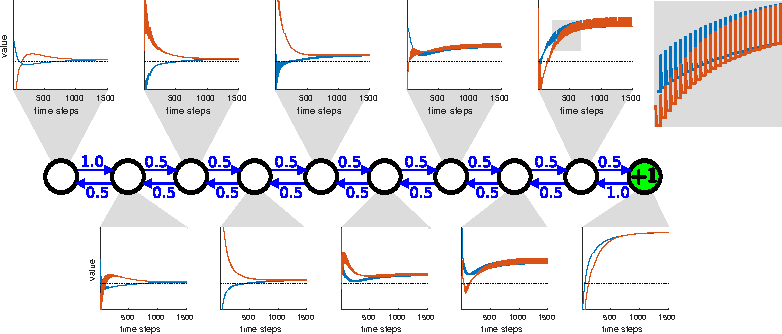
\includegraphics[width=\notesonly{0.9}\slidesonly{0.92}\textwidth]{img/rl_chain_valuecontraction}
		\mode<article>{
		\captionof{figure}{A random walk example in which TD learning will continue fluctuating around the true value but not converge to it.}
		}
	\end{center}

\end{frame}

\subsubsection{Influence of learning rate on TD learning}

\begin{frame}\frametitle{\subsubsecname}

\question{How does the learning rate $\lr$ affect the values obtained through TD learning?}

\mode<presentation>{
	\begin{center}
		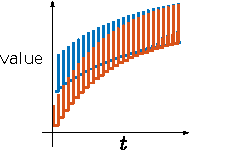
\includegraphics[width=0.3\textwidth]{img/rl_chain_valuecontraction_sub}
	\end{center}
	}
	
\pause

	\begin{itemize}
		\item { large $\eta$: 
			fast learning, large variance (strong fluctuations)}
		\vspace{1mm}
		\item { small $\eta$: 
			slow learning, small variance}
		\vspace{1mm}
		\item { $\eta_{(t)}$ should decay over time, but finding a good annealing schedule may be difficult in practice}
	\end{itemize}

\end{frame}

\subsubsection{Pros \& cons of TD learning}

\begin{frame}\frametitle{\subsubsecname}

\begin{itemize}
\item TD learning learns the value function under policy $\pi$ in an online fashion
\item Every time step updates our guess of the value of one of the states
\end{itemize}

\vspace{10mm}

Pros:
\begin{itemize}
	\item start learning \underline{before} finding out the outcome. We don't have to wait for the reward at the end.
	\item learn online without a final outcome. We can learn from incomplete sequences and non-terminating sequences.
\end{itemize}

Cons:
\pause
\begin{itemize}
	\item biased (we get bad value estimates for states that rarely get sampled and we don't get to choose which state will get sampled next.)
	\item sensitive to the initial state.
\end{itemize}

cf. lecture for more model-free approaches.%: Eligibility Traces \& TD($\lambda$), Batch Value Estimation, ...

\end{frame}


\mode*

\clearpage

\mode<all>
\section{Q-values}

\begin{frame} 
\mode<presentation>{
    \begin{center} \huge
        \secname
    \end{center}  
    }
    \begin{center} 
    values of state-action pairs
    \end{center}
\end{frame}

\begin{frame}

\notesonly{
Another measure use for evaluating policies is the state-action value function, also known as the Q-value function.
We can think of the Q-value function as }a ``higher resolution'' value function. \slidesonly{state value $\rightarrow$ state-action value}

\begin{center}
		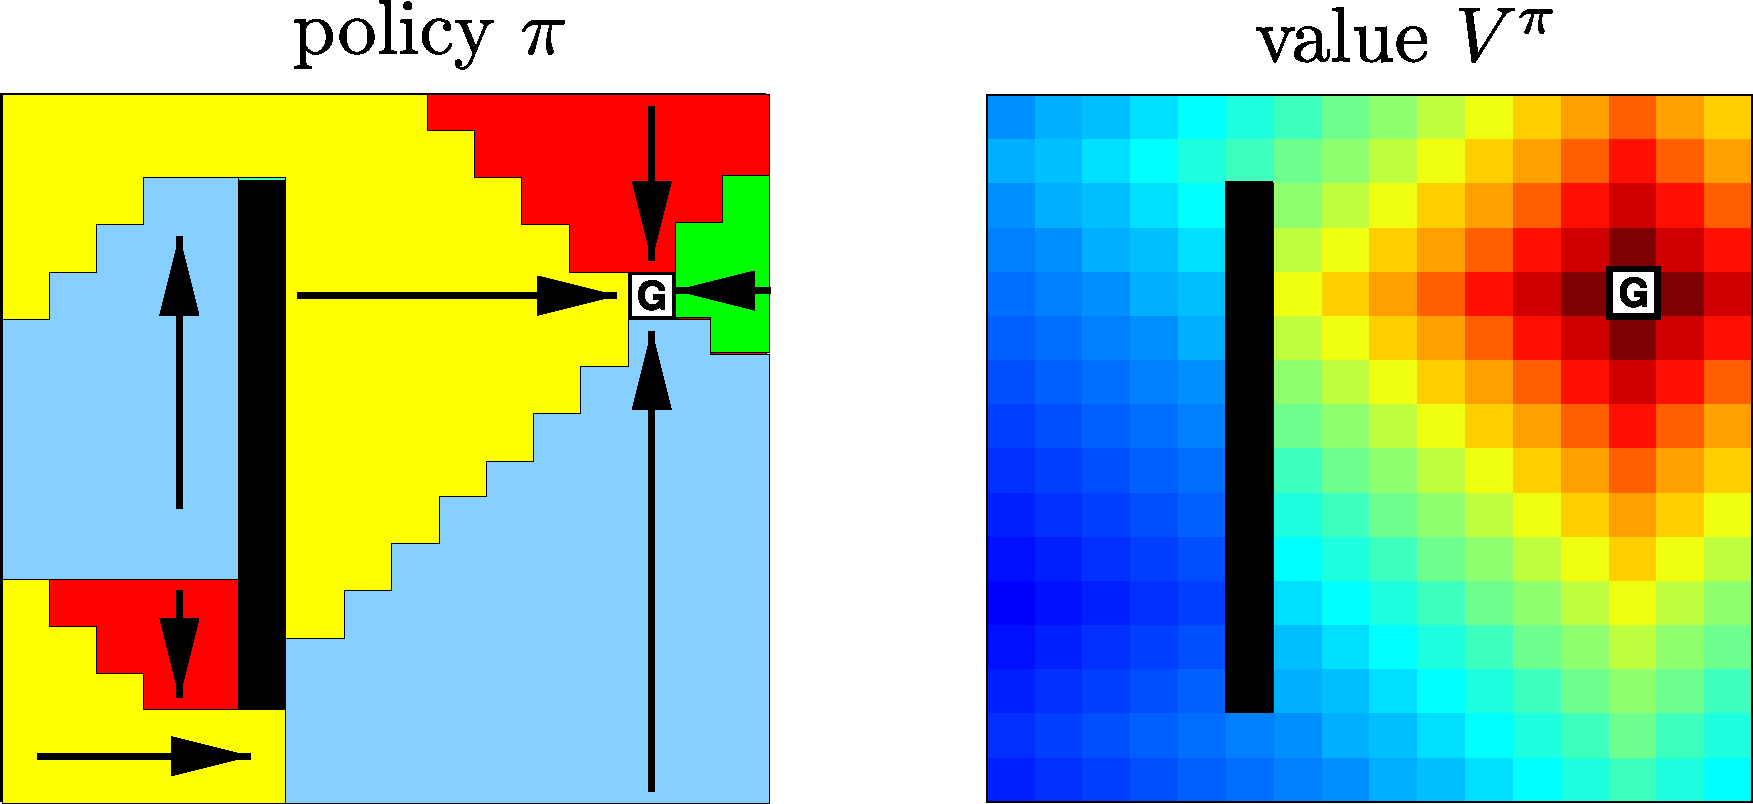
\includegraphics[width=8cm]{img/nav_policy_and_value}
\end{center} 

\begin{center}
		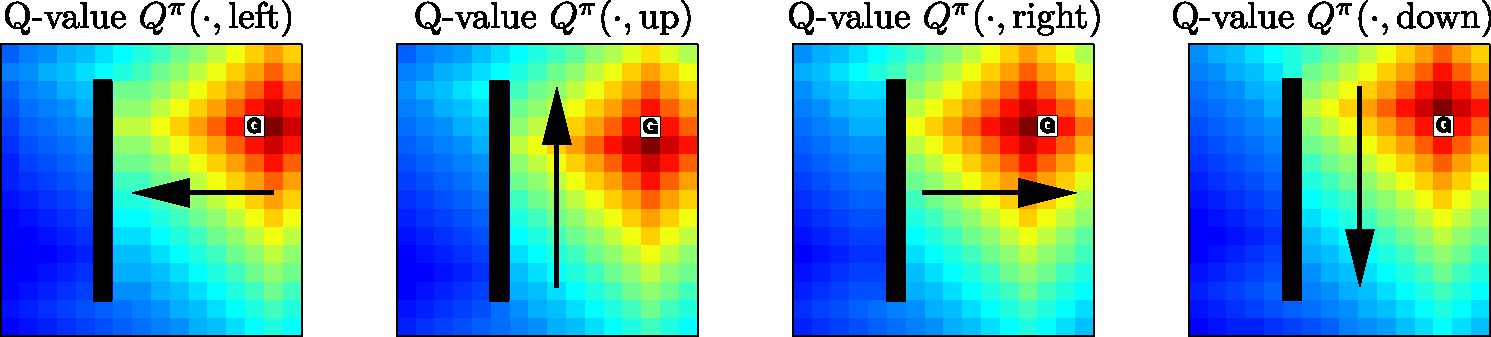
\includegraphics[width=\notesonly{0.9}\textwidth]{img/nav_qvalues}
\end{center} 

\end{frame}

\begin{frame}\frametitle{The Q-value function}

For a fixed policy ${\color{policy}}\pi$, the state-action value function (Q-value function) is defined as:

\begin{equation}
		Q^\pi(\vec x_i, \vec a_k) \quad=\quad 
		\E\bigg\lbrack \,
			\smallsum{t=0}\infty \, \gamma^t \,  
				{\color{reward}r(\vec x^{(t)}, \vec a^{(t)})}
			\, \bigg| \begin{array}{l}
				\scriptstyle \vec x^{(0)} =\, \vec x_i \,, \quad 
					\vec a^{(0)} =\, \vec a_k \\[-1mm]
				\scriptstyle {\color{trans} \vec x^{(t+1)} 
					\,\sim\, P(\cdot|\vec x^{(t)}, \vec a^{(t)})}\\[-1mm]
				\scriptstyle {\color{policy} \vec a^{(t+1)} 
				\,\sim\, \pi(\cdot|{\color{trans}\vec x^{(t+1)}})}
			\end{array}	
		\bigg\rbrack
\end{equation}

The state-action value measures the expected return whenever we start at $\vec x_i$ and take action $\vec a_k$ and follow the policy $\pi$ from there\notesonly{ (cf. \eqref{eq:qbellman})}.

\end{frame}

\begin{frame}

\mode<presentation>{
We have:
\begin{itemize}
\item[] states $\vec x \in \{ \vec x_1, \ldots, \vec x_S\}$, 
actions $\vec a \in \{ \vec a_1, \ldots, \vec a_A\}$,\\
reward function $r(\vec x_i, \vec a_k)$,
\item[]
transition model ${\color{trans} P(\vec x_j | \vec x_i, \vec a_k)}$ and
policy ${\color{policy} \pi(\vec a_k | \vec x_i)}$
\end{itemize}
}

\mode<presentation>{
\begin{center}
		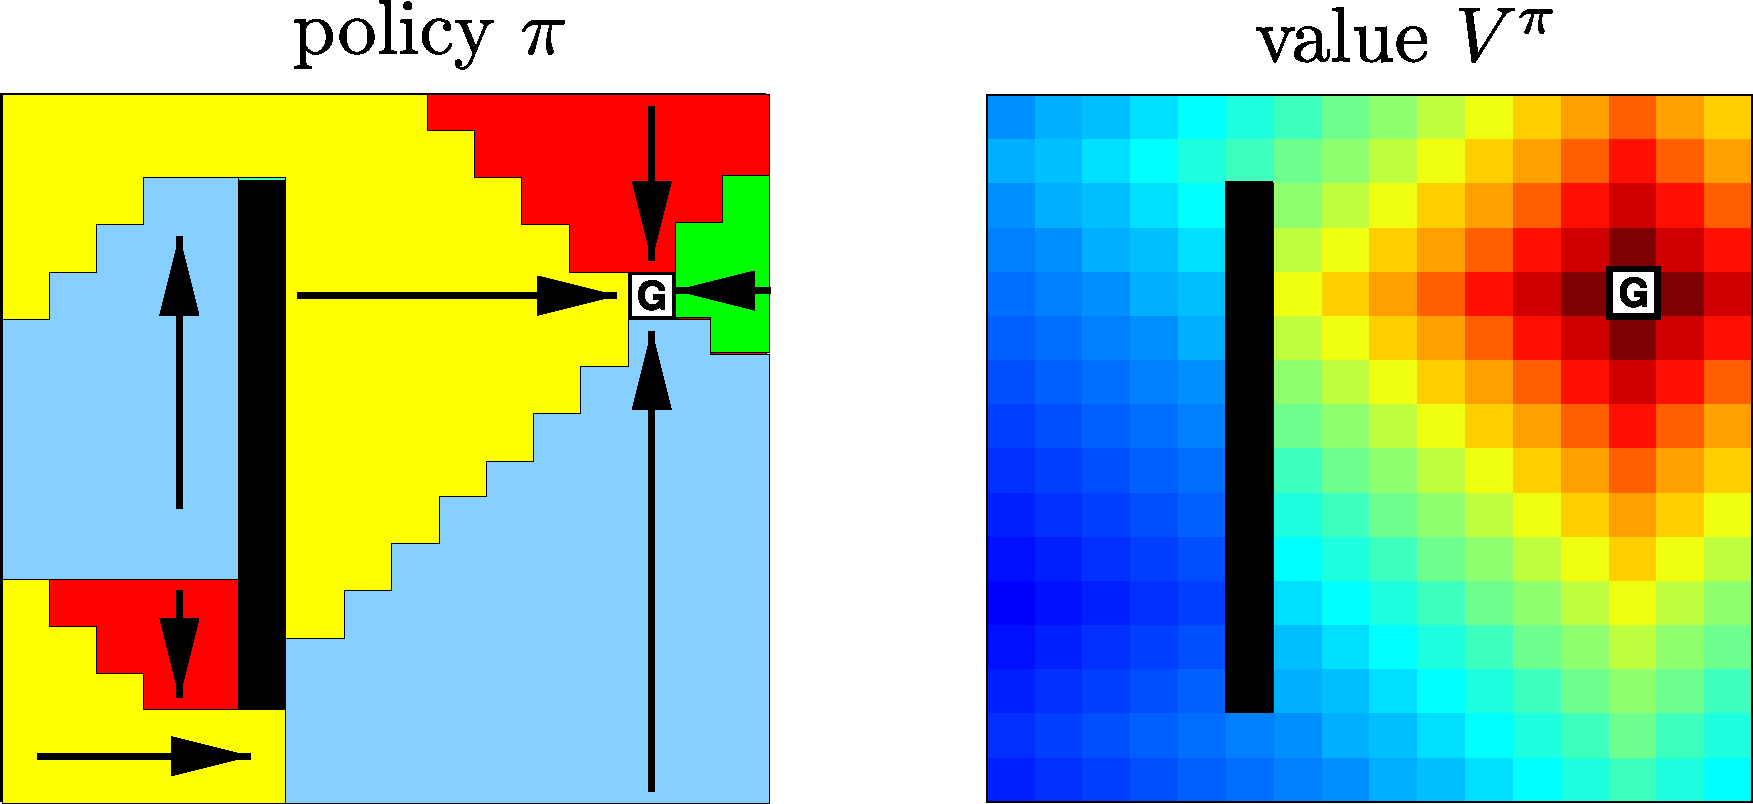
\includegraphics[width=3cm]{img/nav_policy_and_value}
\end{center} 

\begin{center}
		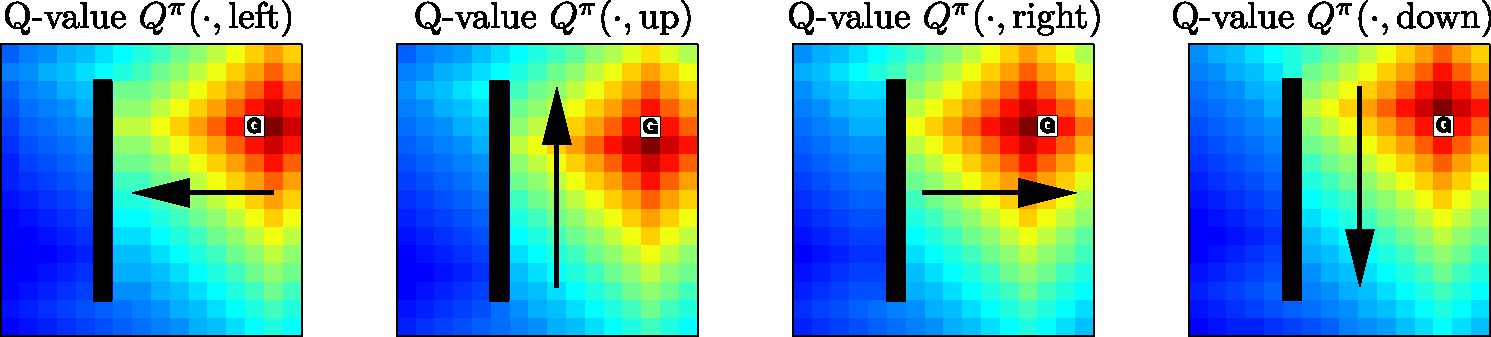
\includegraphics[width=0.7\textwidth]{img/nav_qvalues}
\end{center} 
}

\question{How does the value function relate to the Q-value function?}

\pause

\slidesonly{\vspace{-7mm}}
\notesonly{- yes, through:}

\begin{equation}
V^\pi(\vec x_i) = \visible<3->{
{\only<4>{\color{policy}}\sum_{k=1}^{A}}
}
\visible<4>
{{\color{policy}
\pi(\vec a_k|\vec x_i)
}}
\visible<2->{{\color{black}Q^\pi(\vec x, \vec a_k)}}
\label{eq:vfromq}
\end{equation}

\end{frame}

\begin{frame}
	\only<1,2>{
	\begin{block}{Reminder: Bellman equation (decomposition) for the value function}
			\begin{equation}
			V^\pi_i
			= {\color{reward}\vec r^\pi_i} 
					+ \gamma {\color{trans}\vec P^\pi_{ij}} \vec v^\pi_{j}
			\end{equation} 
	\end{block}
	
	\mode<presentation>{
	Knowing that:\\
	
	Q-values measure the expected return whenever we start at $\vec x_i$ and take action $\vec a_k$ and follow the policy $\pi$ from there
	}
	
	\question{Can we get a similar decomposition for the Q-value function?}
	}
	
	\pause
	
	\begin{block}{Bellman equation (decomposition) for Q-values}
		\vspace{-4mm}	
		\begin{align}
			\label{eq:qbellman}
			Q^\pi(\vec x_i, \vec a_k) \;\;&=\;\; 
			{\color{reward} r(\vec x_i, \vec a_k)} \;+\; 
			\gamma {\color{trans} \sum_{j=1}^S 
				P(\vec x_j | \vec x_i, \vec a_k)} \;
				V^\pi({\color{trans}\vec x_j})
			\slidesonly{\\}
			\notesonly{\intertext{plugging \eqref{eq:vfromq} yields:}}
			&=\;\; 
			{\color{reward} r(\vec x_i, \vec a_k)} \;+\; 
			\gamma {\color{trans} \sum_{j=1}^S 
				P(\vec x_j | \vec x_i, \vec a_k)} \;
				{\color{policy} \sum_{l=1}^{A} \, 
					\pi(\vec a_l | {\color{trans}\vec x_j})} \,
					Q^\pi({\color{trans}\vec x_j}, 
						{\color{policy}\vec a_l})
		\end{align}
	\end{block}
	
	\slidesonly{\vspace{-3mm}}
	
	\notesonly{
	Applying the Bellman decomposition to the Q-value function reveals how Q-values relate to the state-value function.
	}
	
	\only<3->{
	
	\question{What are the implications of having the Bellman decomposition for the Q-value function?}
	
	\pause
	
	- \notesonly{It implies that we can reuse the same policy evaluation methods as we did for the value function that directly operate on the Bellman decomposition (e.g. }model-based methods: analytical solution, fixed-point iteration\notesonly{)}\slidesonly{ for finding the q-value function for some policy}
	
	\question{Can I only reuse model-based evaluation methods to estimate Q-values?}
	
	\slidesonly{\vspace{-3mm}}
	
	- \underline{all} techniques for value estimation apply to Q-values.
	}
	
\end{frame}


\subsection{Finding the optimal policy (recap and extension)}

\subsubsection{Comparing two policies}

\begin{frame}\frametitle{My policy is better than yours (recap)}

\begin{equation}
\pi~
\overset{\mathclap{\substack{%
					\text{``better'' or}\\[1mm]\text{equally ``good''}\\ \big\downarrow
					}}}{{\color{gray}\ge}}
~\pi' 
\quad \text{\textbf{iff}} \quad V^{\pi} (\vec x) \ge V^{\pi'} (\vec x)\,,\quad \forall\; \vec x \in \mathcal{X}
\end{equation}

\end{frame}

\begin{frame}\frametitle{\subsecname}

Recall:
\slidesonly{\vspace{-5mm}}
\begin{equation}
V^{*}(\vec x) = \max_{\pi} V^{\pi} (\vec x)\,,\quad \forall\; \vec x \in \mathcal{X}
\end{equation}

\visible<2-4>{
Similarly for state-action values:

\slidesonly{\vspace{-3mm}}

\begin{equation}
Q^{*}(\vec x, \vec a) = \max_{\pi} Q^{\pi} (\vec x, \vec a)\,,\quad \forall\; \vec x \in \mathcal{X}, \vec a \in \mathcal{A}
\end{equation}
}

\slidesonly{\vspace{-3mm}}

\begin{block}{Optimal Policy}

For all optimal policies $\pi^{*}$:

\slidesonly{\vspace{-3mm}}

\begin{equation}
    V^{\pi^{*}}(\vec x) = V^{*}(\vec x) = \max_{\pi} V^{\pi} (\vec x)\,,\quad \forall\; \vec x \in \mathcal{X}
\end{equation}

A policy $\pi$ that maximizes the value function and yields $\vec v^{*}$ is an optimal policy $\pi^{*}$.\visible<3->{ Consequently, $\forall\; \vec x \in \mathcal{X}, \vec a \in \mathcal{A},$

\only<4>{
\slidesonly{\vspace{-7mm}}
}

\begin{align}
    Q^{\pi^{*}}(\vec x, \vec a) 
    = Q^{*}(\vec x, \vec a) &= \max_{\pi} Q^{\pi} (\vec x, \vec a)\\
    \visible<4>{
    &
    %\kern-2e4\stackrel{\notesonly{\text{with}~\eqref{eq:qbellman}}}{=}
    \overset{\mathclap{\substack{%
    \notesonly{\text{with \eqref{eq:qbellman}}}\vspace{3mm}
					}}}{=}
    {\color{reward} r(\vec x_i, \vec a_k)} \;+\; 
			\gamma {\color{trans} \sum_{j=1}^S 
				P(\vec x_j | \vec x_i, \vec a_k)} \;
				V^*(\vec x_j)
				}
\end{align}


}
    
\end{block}

    
\end{frame}

\begin{frame}\frametitle{Optimal state-action value}

\mode<presentation>{
\begin{equation}
Q^{*}(\vec x, \vec a) = \max_{\pi} Q^{\pi} (\vec x, \vec a)\,,\quad \forall\; \vec x \in \mathcal{X}, \vec a \in \mathcal{A}
\end{equation}
}

\question{How do we interpret $Q^{*}(\vec x, \vec a)$?}\\

\pause

- $Q^{*}(\vec x, \vec a)$ gives us the right action to take to behave optimally in the MDP.

\question{Anything else? How do we extract the policy from the state-action values?}\\

\notesonly{
- Simple readout:
}

\begin{equation}
\pi(\vec a_k | \vec x_i) = \visible<3>{\argmax_{\vec a} Q(\vec x_i, \vec a)}
\end{equation}

\question{Any disadvantages to finding the Q-values directly instead of the value function?}\\

\notesonly{
- The space of the Q-values is proportional to the state space \textbf{as well as} the action space. For a large action space the space of the Q-values would be much larger than that of the state value function.
}

\end{frame}

%\begin{frame} 
%\mode<presentation>{
%switch to lecture slides for
%\vspace{10mm}
    %\begin{center} \large
        %4.2.5 Approximate Reinforcement Learning\\
        %and\\
        %4.2.6 End-to-End RL
    %\end{center}  
    %}
%\vspace{10mm}
    %and hopefully come back
%\end{frame}

\subsection{\notesonly{On-policy} TD learning of Q-values (SARSA)}

% -----------------------------------------------------------------------------
\begin{frame}\frametitle{\subsecname}
	\begin{itemize}
		\item Online learning requires sampling from a long Markov chain:\\
		\begin{center}
			(State$^{(t)}$-Action$^{(t)}$-{\color{reward} Reward$^{(t)}$}-{\color{trans} State$^{(t+1)}$}-{\color{policy} Action$^{(t+1)}$})
		\end{center}
		\vspace{2mm}
		\item This enables the asynchronous on-line update of the value function one state at a time (cf. TD($0$)\notesonly{ in \eqref{eq:tdlearningvalue}})
		
		\slidesonly{\vspace{-7mm}}
		\mode<presentation>{
		\begin{equation}
			\tilde V^{\pi}_{(t+1)}(\vec x^{(t)}) \; = \; 
			\tilde V^{\pi}_{(t)}(\vec x^{(t)}) \;+\;
			\lr \Big( \underbrace{{\color{reward}r^{(t)}} 
			+ \overbrace{
			\gamma \tilde V^{\pi}_{(t)}({\color{trans}\vec x^{(t+1)}})
			}^{\substack{\text{discounted value of}\\ \text{the next step}}} 
			- \tilde V^{\pi}_{(t)}{(\vec x^{(t)})}}_{\text{TD-error }\Delta V_{(t)}} \Big) 
		\end{equation}
		}
		
		\slidesonly{\vspace{-3mm}}
	
		Applying TD learning to Q-values leads to:
		
		\slidesonly{\vspace{-4mm}}
	
		\begin{align}
			\tilde{Q}^\pi_{(t+1)}(\vec x^{(t)},\, \vec a^{(t)} ) &\\
			 = \, \tilde{Q}^\pi_{(t)} ( \vec x^{(t)},\, \vec a^{(t)} )& \, + \, \eta \, \underbrace{ \big( {\color{reward} r^{(t)}} \, + \, \gamma \, \tilde{Q}^\pi_{(t)} ({\color{trans}  \vec x^{(t+1)}},\,{\color{policy}  \vec a^{(t+1)}} ) - \tilde{Q}^\pi_{(t)} ( \vec x^{(t)},\, \vec a^{(t)} ) \big)}_{\Delta Q_{(t)}} \nonumber
		\end{align}
		
		\slidesonly{\vspace{-3mm}}
		
		\item There exists a SARSA($\lambda$) variant with eligibility traces (cf. TD($\lambda$)).
	\end{itemize}

\end{frame}

% -----------------------------------------------------------------------------
\begin{frame} \frametitle{On-policy vs. off-policy estimates}
	\begin{block}{On-policy:}
		Q-values are estimated for the policy, which generates the Markov chain.
	\end{block}
	
	\vspace{5mm}
	
	\begin{block}{Off-policy:}
		Q-values are estimated for a policy $\pi$. The Markov chain is generated by a different policy $\pi'$.
	\end{block}
	
	\mode<presentation>{
	SARSA:
	\begin{align}
			\tilde{Q}^\pi_{(t+1)}(\vec x^{(t)},\, \vec a^{(t)} ) &\\
			 = \, \tilde{Q}^\pi_{(t)} ( \vec x^{(t)},\, \vec a^{(t)} )& \, + \, \eta \, \underbrace{ \big( {\color{reward} r^{(t)}} \, + \, \gamma \, \tilde{Q}^\pi_{(t)} ({\color{trans}  \vec x^{(t+1)}},\,{\color{policy}  \vec a^{(t+1)}} ) - \tilde{Q}^\pi_{(t)} ( \vec x^{(t)},\, \vec a^{(t)} ) \big)}_{\Delta Q_{(t)}}
	\end{align}
	}
	
	SARSA estimates the Q-values for a fixed policy which generates the Markov chain. Therefore, SARSA is on-policy
\end{frame}

\subsection{Off-policy TD learning of Q-values}

% -----------------------------------------------------------------------------
\begin{frame}{Only} \frametitle{\subsecname}
	
	TD learning of Q-values in general:
	\begin{equation}
			\tilde{Q}^\pi_{(t+1)}\notesonly{(\vec x^{(t)},\, \vec a^{(t)} )}
			\,= \,
			\tilde{Q}^\pi_{(t)}\notesonly{ ( \vec x^{(t)},\, \vec a^{(t)} )} \, + \, \eta \, {\color{magenta}\Delta Q_{(t)}}
	\end{equation}
	
	\only<1>{
		\slidesonly{
		\vspace{30mm}
		}
	When going from on to off-policy, what changes is that the actions that lead to the next state are sampled using a \textbf{different} \emph{sampling} policy $\pi'$\\
		\begin{equation}
		\vec a^{(t)} \sim \pi'(\vec a | \vec x^{(t)})
		\end{equation}
		\slidesonly{
		\vfill
		}
		}
	
	\notesonly{In the case of TD learning, on- or off-policy becomes apparent from ${\color{magenta}\Delta Q_{(t)}}$:}
	
	\begin{itemize}
		\item<only@2> On-policy TD learning of Q-values (SARSA):
		
		\begin{equation}
				{\color{magenta}\Delta Q_{(t)}} \,=\, {\color{reward} r^{(t)}} \, + \, \gamma \, \overbrace{\tilde{Q}^\pi_{(t)} ({\color{trans}  \vec x^{(t+1)}},\,{\color{policy}  \vec a^{(t+1)}} )}^{\circledast} - \tilde{Q}^\pi_{(t)} ( \vec x^{(t)},\, \vec a^{(t)} )
				\label{eq:deltaqONpolicy}
		\end{equation}
		
		\item<only@2,3> Off-policy TD learning of Q-values:
		
		\slidesonly{\vspace{-5mm}}
		
		\begin{equation}
					{\color{magenta}\Delta Q_{(t)}} \,=\, {\color{reward}r^{(t)}} 
				 \, + \, \gamma \, \overbrace{{\color{policy}\smallsum{k=1}{A}
					\pi(\vec a_k \,|\, {\color{trans}\vec x^{(t+1)}})} \,
					Q({\color{trans}\vec x^{(t+1)}}, {\color{policy}\vec a_k})}^{\circledast} 
				\;-\; Q(\vec x^{(t)}, \vec a^{(t)})
				\label{eq:deltaqOFFpolicy}
		\end{equation}
		
		\notesonly{In both \eqref{eq:deltaqONpolicy} and \eqref{eq:deltaqOFFpolicy}, the }$\circledast$ represents the discounted value of the next step.
		
		\notesonly{What is happening \eqref{eq:deltaqOFFpolicy} is that the discounted value\notesonly{\footnote{in this particular case, the value is the state-action value, but TD learning can be applied to estimating the state value function just as well.}} of the next step is weighted by the probability of the action being sampled by the policy $\pi$ which is being evaluated as it may differ from the sampling policy $\pi'$.}
		
	\item<only@3> Advantage of off-policy: Data (i.e. Markov chains) can be reused as the policy ${\color{policy}\pi}$, the one we want to optimize, changes (e.g. policy iteration)
	\item<only@3> contracts for ergodic Markov chain, i.e.
	\begin{equation}
	\lim\limits_{p\to\infty} \E\Big\lbrack
				\smallsum{t=0}{p} \Delta Q_{(t)} 
			\Big\rbrack= Q^{\pi}
	\end{equation}
	
	\end{itemize}
	
\end{frame}




\mode*

\clearpage

\mode<all>
\section{Policy Improvement}

\begin{frame} 
\mode<presentation>{

	\svspace{10mm}
    \begin{center} \huge
        \secname
    \end{center}  
    
    \begin{center}
    updating the policy to yield a better state value function and state-action value function
    \end{center}
    
	\svspace{10mm}
    \begin{center}
		
\includegraphics[width=0.2\textwidth]{img/meme_givebetterpolicy}
    \end{center}
    }
\end{frame}

\subsection{Greedy policy}

\begin{frame}\frametitle{\secname:~\subsecname}

\only<1>{
	The optimal policy is found by:

	\begin{align}
	\pi^* = \argmax_{\pi} V^\pi(\vec x) = \argmax_{\pi} Q^\pi(\vec x, \vec a)\\
	\end{align}

	The above boils down to selecting the best action when at some state $\vec x$:

	\begin{equation}
		\vec a_l = \argmax_{1\leq k \leq A} Q^\pi(\vec x_i, \vec a_k)
	\end{equation}
}
\only<2,3>{
	The greedy\footnote{``greedy'' is to try and get closer to the ``globally'' optimal choice by making ``locally'' optimal decisions} policy method decides on a new policy $\pi'$ using the Q-value function, by:	

	\begin{equation}
	   \pi'(\vec a_k | \vec x_i) = \left\{
	   \begin{array}{ll}
		 1, &\text{if } k = \argmax_{1 \leq l \leq A} Q^\pi(\vec x_i, \vec a_l) \\
		 0, &\text{else.}
	   \end{array}
	   \right.
	\end{equation}
}
\only<3>{
\mode<presentation>{
\begin{center}
		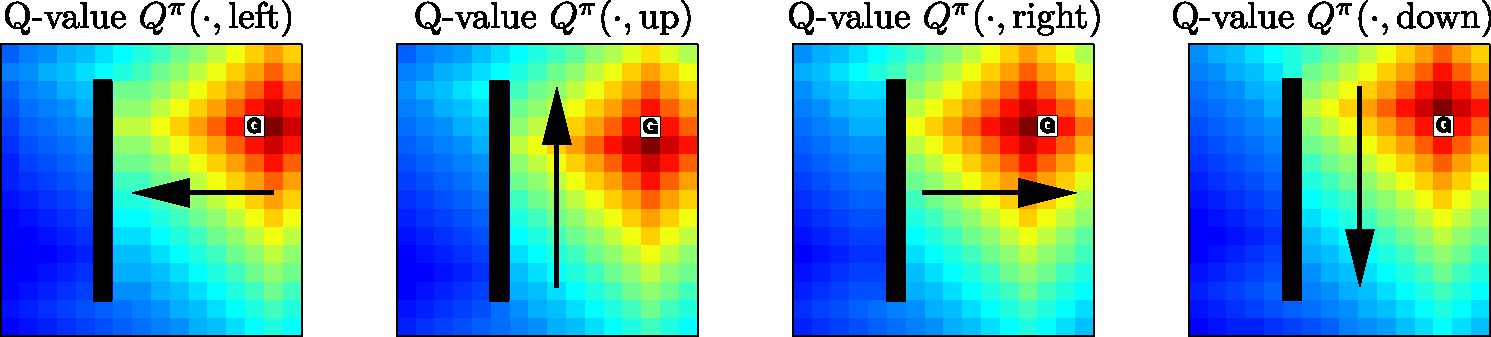
\includegraphics[width=\notesonly{0.9}\textwidth]{img/nav_qvalues}
\end{center} 
}
}

\end{frame}

\subsection{Policy improvement theorem}

% -----------------------------------------------------------------------------
\begin{frame}[label=policy_improvement] \frametitle{\subsecname}
	\begin{itemize}
		\item A policy $\pi'$ is equal or better than a policy $\pi$, i.e.
			\begin{equation*}
				V^{\pi'}(\vec x) \geq V^\pi(\vec x)
			\end{equation*}
			for all states $\vec x$, if:
			\begin{equation*}
				Q^\pi \left(\vec x, \vec a^{\pi'}_{(\vec x)} \right) \geq V^\pi(\vec x)
			\end{equation*}
		\vspace{2mm}		
		\item $Q^\pi \left(\vec x, \vec a^{\pi'}_{(\vec x)} \right)$ is the value of action $\vec a^{\pi'}_{(\vec x)}$ according to policy $\pi'$ at $\vec x$\\[3pt] when following policy $\pi$ afterwards
	\end{itemize}
	
	%\blfootnote{\hfill\hyperlink{policy_improvement_proof}{\beamerbutton{derivation here}}}
\end{frame}

\subsection{Policy iteration}

% -----------------------------------------------------------------------------
\begin{frame} \frametitle{\subsecname}
		\vspace{1mm}
		\small
		\mbox{
		\hspace{-4mm}
		Any policy $\pi_i$ is {\em improved} by
			the greedy policy $\pi_{i+1}$ operating on $\pi_i$'s Q-values $Q^{\pi_i}$:}
			\vspace{1mm}	
			\begin{align*}
				V^\pi(\vec x_i) &= \sum_{k=1}^{A} \pi(\vec a_k | \vec x_i) \; Q^\pi(\vec x_i, \vec a_k) \\
				&\leq \max_k Q^\pi(\vec x_i, \vec a_k) \overset{!}{=} Q^\pi \left(\vec x, \vec a^{\pi'}_{(\vec x)} \right)
			\end{align*}
		%\vspace{4mm}
		%\item alternating value estimation and policy improvement 
		\normalsize
	\vspace{4mm}
	\begin{block}{Policy iteration (PI)}
		initialize policy $\pi_{0}$ randomly\\
		\While{Q-values not converged}{
			estimate 
				%(with any algorithm) Q-value function 
				$\tilde Q^{\pi_i} :\approx Q^{\pi_i}$ of policy $\pi_i$ (estimation of Q-values via e.g. SARSA for $\pi_i$)\\
			choose $\pi_{i+1}$ to be the greedy policy on $\tilde Q^{\pi_i}$
		} 
		
		\vspace{-4mm}
		{\footnotesize\hfill\citep[see]%
		[for convergence with estimated Q-values]{Bertsekas07}}
	\end{block}	
\end{frame}

\subsection{On-line off-policy improvement: Q-learning}

\begin{frame}\frametitle{\subsecname}

Q-learning is an on-line off-policy improvement method, which integrates greedy policy improvement into off-policy TD learning.

\begin{block}{Q-learning}
	Pick a sampling policy $\pi$. (It will typically depend on the current Q-values.)
	\slidesonly{\vspace{-3mm}}
	\begin{align}
			\tilde Q_{(t+1)}^*(\vec x^{(t)}, \vec a^{(t)})
			\;\;=\;\;&
			\tilde Q_{(t)}^*(\vec x^{(t)}, \vec a^{(t)})
			\\
			&\kern-10ex
			 \;+\; \lr \Big( \underbrace{
				{\color{reward}r^{(t)}} + \gamma 
				\overbrace{
					{\color{policy} \max_{1 \leq k\leq A}}
					\tilde Q_{(t)}^*({\color{trans}\vec x^{(t+1)}}, 
						{\color{policy}\vec a_k})
				}^{\text{\scriptsize \kern-2exgreedy policy improvement\kern-2ex}}
				- \, \tilde Q_{(t)}^*(\vec x^{(t)}, \vec a^{(t)})	
				}_{\text{\scriptsize TD-error} \displaystyle \scriptstyle \;\Delta Q_{(t)} }\Big)
	\end{align}
\end{block}
	
	\only<1>{
	$\Delta Q_{(t)}$ in SARSA for comparison:
	\begin{equation}
			\Delta Q_{(t)} = {\color{reward} r^{(t)}} \, + \, \gamma \, \tilde{Q}^\pi_{(t)} ({\color{trans}  \vec x^{(t+1)}},\,{\color{policy}  \vec a^{(t+1)}} ) - \tilde{Q}^\pi_{(t)} ( \vec x^{(t)},\, \vec a^{(t)} )
	\end{equation}
	}
	\only<2>{
	
	\slidesonly{\vspace{-3mm}}
	
	\question{How do we extract the optimal policy $\pi^*$?}\\
	
	\slidesonly{\vspace{-5mm}}
	
	\notesonly{
	 - Extracting the optimal policy is done the same way as by the greedy policy:
	 }
	\begin{equation}
	   \pi^*(\vec a_k | \vec x_i) = \left\{
	   \begin{array}{ll}
		 1, &\text{if } k = \argmax_{1 \leq l \leq A} Q^*(\vec x_i, \vec a_l) \\
		 0, &\text{otherwise.}
	   \end{array}
	   \right.
	\end{equation}
	}

\end{frame}

\begin{frame}\frametitle{\subsecname}

Q-learning \citep{Watkins92}:
\begin{itemize}
\item online policy improvement
\item estimates the Q-value function of an optimal (unknown) policy $\pi^*$
\item off-policy with sampling policy $\pi$
\item effectively TD learning with greedy policy improvement
\item Q-learning is a contraction mapping for \emph{any} ergodic Markov chain
			\begin{equation}
				\lim\limits_{p \to \infty} \E \Big\lbrack
					\smallsum{t=0}{p} \Delta Q_{(t)} \Big\rbrack
				= Q^{\pi^*}
			\end{equation}
\item Q-learning is the only on-line off-policy algorithm for policy improvement.
\end{itemize}

\end{frame}

\mode*

\clearpage

\mode<all>
\section{Exploration vs. Exploitation}

\begin{frame} 
\mode<presentation>{
    \begin{center} \huge
        \secname
    \end{center}  
    \vspace{5mm}
    }
	\begin{table}[h]
	\centering
	\resizebox{0.8\textwidth}{!}{%
	\begin{tabular}{ccc}
	exploration                                                                               &  & exploitation                                                                                                         \\
	\multicolumn{3}{c}{$\xleftrightarrow{\hspace*{5cm}}$}                                                                                                                                                                               \\
	\begin{tabular}[c]{@{}c@{}}visit all state-action pairs\\ sufficiently often\end{tabular} & \hspace{2cm} & \begin{tabular}[c]{@{}c@{}}converge fast and generate\\ as much reward as possible\\ \\ (greedy policy)\end{tabular}
	\end{tabular}%
	}
\end{table}
	
\mode<presentation>{
%\begin{center}
		%
\includegraphics[width=2cm]{img/explore}
%\end{center} 
%\begin{table}[]
%\centering
%\resizebox{0.2\textwidth}{!}{%
%\begin{tabular}{|c|c|c|}
%\hline
 %&                   &                       \\  \hline
 %& &  \\ \hline
 %&                       &                       \\ \hline
%\end{tabular}%
%}
%\end{table}
	%\slidesonly{\textbf{(see blackboard)}}
}
\end{frame}

\subsection{Finding a balance}

\begin{frame}\frametitle{\subsecname}


Some of the possible approaches:
\begin{enumerate}

	\item parametrize the extraction of the policy from the Q-values:
	
		%\begin{enumerate}[a\notesonly{.}]
		\begin{itemize}
		
		\item $\varepsilon$-greedy\only<2>{:

			\begin{equation}
			   \begin{array}{cc}
				 &\varepsilon\text{-greedy}\\
				 &\text{policy}
			   \end{array}
			   \pi(\vec a_k | \vec x_i) = \left\{
			   \begin{array}{ll}
				 {1-\varepsilon}, &\text{if } k = \argmax_{1 \leq l \leq A} Q(\vec x_i, \vec a_l) \\
				 {\frac{\varepsilon}
				 {A-1}}, &\text{otherwise.}
			   \end{array}
				 \right.
			\end{equation}
			
			\question{How does $\varepsilon$ control the balance?}
			}
			
		%\item 
		
		%\begin{equation}
			%\pi(\vec a_k \,|\, \vec x_i) 
				%\quad=\quad 
				%\frac{\exp\big( \beta \, Q(\vec x_i, \vec a_k)\big)}
				%{\sum_{l=1}^A \exp\big( \beta \, Q(\vec x_i, \vec a_l) \big)}
		%\end{equation}
		

		%\end{enumerate}
		\end{itemize}

	\item Optimistic Initialization
	
	\only<3>{
	A greedy sampling policy would fail at exploration,\\
	unless all Q-values are initialized with high values.
	
	\begin{itemize}
		\item initializing all Q-values with high 
			$Q_{(0)} \geq \frac{r_\text{max}}{1-\gamma}$ directs exploration
		\vspace{1mm}
		\item unexplored actions are initially made very attractive
		
		\question{How does the transition to exploration happen?}\\
		
		\notesonly{
		- Through experience, as Q-values are reduced over time exploitation takes over.
		}
	\end{itemize}
	}


\end{enumerate}

\end{frame}


\mode*

%\clearpage

\section{References}
\begin{frame}[allowframebreaks] \frametitle{References}
	\scriptsize
	\bibliographystyle{plainnat}
	\bibliography{bibliography}
\end{frame}

\end{rightcolumn}
\end{paracol}

\end{document}
